\documentclass{standalone}
\usepackage{tikz}
\usetikzlibrary{shapes.geometric}
\newcommand{\repeater}[3]{%
 \node ({#1}) at ({#2}) {%
  \begin{tikzpicture}%
   \draw [black,thick] (-.25,0) -- (0,0.5) -- (0.25,0) -- (-0.25,0);%
   \draw [black,thick,domain=-45:225] plot ({0.2*cos(\x)}, {0.5+0.2*sin(\x)});%
   \draw [black,thick,domain=-45:225] plot ({0.4*cos(\x)}, {0.5+0.4*sin(\x)});%
   \node (xxx) at (0,-.2) {{#3}};%
  \end{tikzpicture}%
 } %
}

\newcommand{\activerepeater}[3]{%
 \node ({#1}) at ({#2}) {%
  \begin{tikzpicture}%
   \draw [black,thick] (-.25,0) -- (0,0.5) -- (0.25,0) -- (-0.25,0);%
   \draw [red,thick,domain=-45:225] plot ({0.2*cos(\x)}, {0.5+0.2*sin(\x)});%
   \draw [red,thick,domain=-45:225] plot ({0.4*cos(\x)}, {0.5+0.4*sin(\x)});%
   \node (xxx) at (0,-.2) {{#3}};%
  \end{tikzpicture}%
 } %
}


\newcommand{\user}[3]{%
 \node ({#1}) at ({#2}) {%
  \begin{tikzpicture}%
   \draw [black,fill=black] (-.25,0) -- (0,0.5) -- (0.25,0) -- (-0.25,0);%
   \draw [black,fill=black] (0,.5) circle (.2); %
   \node (xxx) [text width=0.6cm, align=center] at (-.35cm,-.4) {{#3}};%
  \end{tikzpicture}%
 } %
}

\newcommand{\activeuser}[3]{%
 \node ({#1}) at ({#2}) {%
  \begin{tikzpicture}%
   \draw [red,fill=red] (-.25,0) -- (0,0.5) -- (0.25,0) -- (-0.25,0);%
   \draw [red,fill=red] (0,.5) circle (.2); %
   \node (xxx) [text width=0.6cm, align=center] at (-.35cm,-.4) {{#3}};%
  \end{tikzpicture}%
 } %
}

\begin{document}
  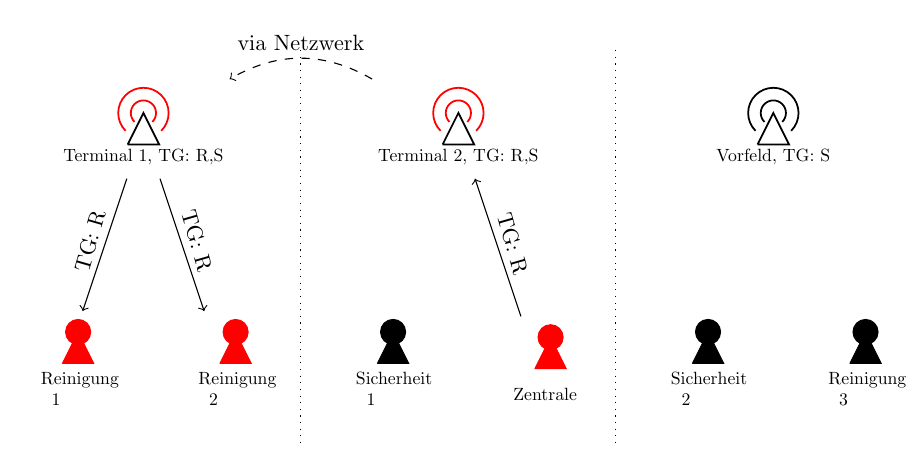
\begin{tikzpicture}[every node/.style={scale=.8}]
   \activeuser{r1}{ 0,0}{Reinigung 1};
   \activeuser{r2}{ 2,0}{Reinigung 2};	
   \draw[dotted] (3,4) -- (3,-1);
   \user{s1}{ 4,0}{Sicherheit 1};
   \activeuser{z} { 6,0}{Zentrale};
   \draw[dotted] (7,4) -- (7,-1);
   \user{s2}{ 8,0}{Sicherheit 2};
   \user{r3}{10,0}{Reinigung 3};
   \activerepeater{R1}{1,3}{Terminal 1, TG: R,S};
   \activerepeater{R2}{5,3}{Terminal 2, TG: R,S};
   \repeater{R3}{9,3}{Vorfeld, TG: S};
   \draw[->] (z) -- node[above,rotate=-74] {TG: R} (R2);
   \path[->,dashed] (R2) edge [bend right] node[above] {via Netzwerk} (R1);
   \draw[->] (R1) -- node[above,rotate=74] {TG: R} (r1);
   \draw[->] (R1) -- node[above,rotate=-74] {TG: R} (r2);
  \end{tikzpicture}
\end{document}
